\documentclass[12pt,norsk,a4paper]{article}
\usepackage{babel}
\usepackage[utf8]{inputenc}
\usepackage{amsmath}
\usepackage{amssymb}
%\usepackage{calc}
\usepackage{graphicx}
\usepackage{float}
\usepackage{color}
\usepackage{physics}
\usepackage{listings}
\usepackage{siunitx}
\usepackage{todonotes}
\usepackage[version=4]{mhchem}
\usepackage{hyperref}
\usepackage{multirow}
\usepackage{tikz}
\usepackage{mhchem}
\usepackage{pdfpages}
\usepackage[margin=1.3cm, includeheadfoot]{geometry}
\usepackage{listings}
\usepackage{xcolor}
\lstset { %
    language=C++,
    backgroundcolor=\color{black!5}, % set backgroundcolor
    basicstyle=\footnotesize,% basic font setting
}
\newcommand{\RN}[1]{%
	\textup{\uppercase\expandafter{\romannumeral#1}}%
}
\renewcommand{\exp}[1]{\mathrm{e}^{#1}}



%reference
%\usepackage{biblatex}
%\addbibresource{sources.bib}
%to here

%for text boxes
\usepackage{fancybox}
\usepackage{framed}
\usepackage{color}
\definecolor{shadecolor}{rgb}{1,0.8,0.3}
%to here




\definecolor{codegreen}{rgb}{0,0.6,0}
\definecolor{codegray}{rgb}{0.5,0.5,0.5}
\definecolor{codepurple}{rgb}{0.58,0,0.82}
\definecolor{backcolour}{rgb}{0.95,0.95,0.92}
\lstset{showstringspaces=false,
	basicstyle=\ttfamily,
	keywordstyle=\color{codegreen},
	commentstyle=\color{magenta},
	numberstyle=\tiny\color{codegray},
	stringstyle=\color{codepurple},
	breaklines=true,
	literate={0}{{\textcolor{blue}{0}}}{1}%
	{1}{{\textcolor{blue}{1}}}{1}%
	{2}{{\textcolor{blue}{2}}}{1}%
	{3}{{\textcolor{blue}{3}}}{1}%
	{4}{{\textcolor{blue}{4}}}{1}%
	{5}{{\textcolor{blue}{5}}}{1}%
	{6}{{\textcolor{blue}{6}}}{1}%
	{7}{{\textcolor{blue}{7}}}{1}%
	{8}{{\textcolor{blue}{8}}}{1}%
	{9}{{\textcolor{blue}{9}}}{1}%
	{.0}{{\textcolor{blue}{.0}}}{2}% Following is to ensure that only periods
	{.1}{{\textcolor{blue}{.1}}}{2}% followed by a digit are changed.
	{.2}{{\textcolor{blue}{.2}}}{2}%
	{.3}{{\textcolor{blue}{.3}}}{2}%
	{.4}{{\textcolor{blue}{.4}}}{2}%
	{.5}{{\textcolor{blue}{.5}}}{2}%
	{.6}{{\textcolor{blue}{.6}}}{2}%
	{.7}{{\textcolor{blue}{.7}}}{2}%
	{.8}{{\textcolor{blue}{.8}}}{2}%
	{.9}{{\textcolor{blue}{.9}}}{2}%
}




\begin{document}
\author{Thomas Aarflot Storaas and Erik Fagerås Skaar\\
	Department of Chemistry\\
	University of Oslo\\	
}

\title{Project 1}
\maketitle

\section{Abstract}
In this article the numerical approximation to a one dimensional Poisson equation is studied. Three approaches are taken. One with a straight forward Gaussian elimination in a general form. One in a specified gaussian elimination form. The third approach are done with LU decomposition using the libarary "Armadillo". The numerical accuracy is then analysed and the three methods are then compared with respect to FLOPS and time used. All the code can be found at \href{https://github.com/erikfsk/Project-1}{https://github.com/erikfsk/Project-1}. %\cite{Armadillo}


\section{Underlying theory}

The Poisson's equation is a classical equation from electromagnetism, which states that $\nabla^2\Phi=-4\pi\rho(\mathbf{(r)})$. The electrostatic potential $\Phi$ is a sentro- symmetrical potential, which makes it possible to rewrite the potential as a one dimentional equation with respect to the distance from origo, $\mathbf{r}$.
\begin{align*}
	\frac{1}{r^2}\pdv{r}\qty(r^2 \pdv{\Phi}{r})=-4\pi\rho(r)
\end{align*}
Introducing the substitutions $\Phi(r)=\phi(r)/r$ gives:
\begin{align}
	\pdv[2]{\phi}{r}=-4\pi r \rho(r)
\end{align}

Further manipulation of the expression with letting $x\to  u$ and $r\to x$ gives:
\begin{align*}
	-u''(x)=f(x)
\end{align*}

For this project the Poisson equation will be solved with Dirichlet boundary conditions and source function $f(x)=100\exp{-10x}$, in the interval $x\in[0,1]$, which gives.
\begin{align}
	u(0)=u(1)=0
\end{align}\label{2}
For this specific source function a numerical solution can be found by doing a double integration, and using the Dirichlet boundary conditions. 
\begin{align*}
	f(x)&=100\exp{-10x}\\
	\int f(x)\dd[2]{x}&=c_1x+c_2 + e^{-10 x}\\
	&=1-\qty(1-\exp{-10})x-\exp{-10x}
\end{align*}

The discretized approximation to $u$ is $v_i$, where the step size is defined as $h=1/(n+1)$ with grid points(sample step) $x_i=ih$. The discretized approximation from $\ref{2}$ gives $v_0=v_{n+1}=0$. The second derivative approximation of $u$ are
\begin{align*}
	&f_i=-\frac{v_{i+1}+2v_{i}-{v_{i-1}}}{h^2}&i=1,2...n
\end{align*} 

For each step $x_i$ a equation can be found:

\begin{align*}
	f_2=(-v_{1}+2v_{2}-v_{3})/h^2\\
	f_3=(-v_{2}+2v_{3}-v_{4})/h^2\\
	f_4=(-v_{3}+2v_{4}-v_{5})/h^2\\
\end{align*}

Note here that the end points are not included. This system of equations can be organized in a matrix, by defining $\tilde{b}_i=h^2f_i$.
\begin{align*}
	\begin{array}{cccc}
	2 & -1 & 0 & 0 \\ 
	-1 & 2 & -1 & 0 \\ 
	0 & -1 & 2 & -1 \\ 
	0 & 0 & -1 & 2
	\end{array}
\end{align*}
 A row reduction of $A\mathbf{x}=f$ will give the solution to all the equations.


\section{Method}

\subsection*{General Gaussian elimination}

The matrix equations we need to solve is the following:

\begin{align*}
	\mathbf{A} = \begin{bmatrix}
	b_1& c_1 & 0 &\dots   & \dots &\dots \\
	a_1 & b_2 & c_2 &\dots &\dots &\dots \\
	& a_2 & b_3 & c_3 & \dots & \dots \\
	& \dots   & \dots &\dots   &\dots & \dots \\
	&   &  &a_{n-2}  &b_{n-1}& c_{n-1} \\
	&    &  &   &a_{n-1} & b_n \\
	\end{bmatrix}\begin{bmatrix}
	v_1\\
	v_2\\
	\dots \\
	\dots  \\
	\dots \\
	v_n\\
	\end{bmatrix}
	=\begin{bmatrix}
	\tilde{b}_1\\
	\tilde{b}_2\\
	\dots \\
	\dots \\
	\dots \\
	\tilde{b}_n\\
	\end{bmatrix}
\end{align*}

Applying a general approach to the gaussian elimination of a $4\cross4$ matrix gives an expression which can be generalized:

\begin{align*}
\begin{bmatrix}
b_1 & c_1 & 0 & 0 \\ 
a_1 & b_2 & c_2 & 0 \\ 
0 & a_2 & b_3 & c_3 \\ 
0 & 0 & a_3 & b_4
\end{bmatrix}\begin{bmatrix}
\tilde{b}_1 \\ 
\tilde{b}_2 \\ 
\tilde{b}_3 \\ 
\tilde{b}_4
\end{bmatrix}\to
\begin{bmatrix}
1 & c_1/b_1 & 0 & 0 \\ 
0 & b_2-(c_1/b_1)a_2 & c_2 & 0 \\ 
0 & a_2 & b_3 & c_3 \\ 
0 & 0 & a_3 & b_4
\end{bmatrix}\begin{bmatrix}
\tilde{b}_1/b_1 \\ 
\tilde{b}_2-(\tilde{b}_1/b_1)a_1 \\ 
\tilde{b}_3 \\ 
\tilde{b}_4
\end{bmatrix}
\end{align*}
Note that i have scaled the first row, this is done in a separate step in the code. One more row reduction gives the second row:

\begin{align*}
\begin{bmatrix}
1 & c_1/b_1 & 0 & 0 \\ 
0 & 1 & c_2/(b_2-(c_1/b_1)a_2) & 0 \\ 
0 & a_2 & b_3 & c_3 \\ 
0 & 0 & a_3 & b_4
\end{bmatrix}
\begin{bmatrix}
\tilde{b}_1/b_1 \\ 
(\tilde{b}_2-(\tilde{b}_1/b_1)a_1)/(b_2-(c_1/b_1)a_2)\\ 
\tilde{b}_3 \\ 
\tilde{b}_4
\end{bmatrix}\to\\
\begin{bmatrix}
1 & c_1/b_1 & 0 & 0 \\ 
0 & 1 & c_2/(b_2-(c_1/b_1)a_2) & 0 \\ 
0 & 0 & b_3-c_2\cdot a_2/(b_2-(c_1/b_1)a_2) & c_3 \\ 
0 & 0 & a_3 & b_4
\end{bmatrix}
\begin{bmatrix}
\tilde{b}_1/b_1 \\ 
a_2(\tilde{b}_2-(\tilde{b}_1/b_1)a_1)/(b_2-(c_1/b_1)a_2)\\ 
\tilde{b}_3-a_2(\tilde{b}_2-(\tilde{b}_1/b_1)a_1)/(b_2-(c_1/b_1)a_2) \\ 
\tilde{b}_4
\end{bmatrix}
\end{align*}


From this a general result can be drawn. The next line is always dependent upon the previous lines result. 
Let $d_i$ denote the previous lines result, and $v_i$ denote the previous $\tilde{b}_i$ result. Then a general case can be written as:

\begin{align}
	d_i=b_i-\frac{c_i}{d_{i-1}}a_i\label{di}
\end{align}

\begin{align}
	v_i=\frac{b_i-v_{i-1}a_i}{d_i}\label{vi}
\end{align}


\subsection{Specific Gaussian elimination}

When we have the general Gaussian elimination, we simple take out anything that is unnecessary to calculate. For example we don't need to the a-vector. Simply because it will become zero. And for the backward substitution we don't need to calculate the c-vektor. Same reason as for the a-vector.  

\subsection{LU decomposition}
Test


\subsection{Error}
Test

















\section{Result}


\subsection{General Gaussian elimination}
The general Gaussian elimination implementation is showed below. 

\begin{lstlisting}
    //forward substitution
    for (int i = 1; i<n;i++){
        double alpha = a[i]/b[i-1];
        a[i] = a[i] - alpha*b[i-1];
        b[i] = b[i] - alpha*c[i-1];
        f_tilde[i] = f_tilde[i] - alpha*f_tilde[i-1];
    }

    //backward substitution
    for (int i = n-2; i>-1;i--){
        double c_ledd = c[i]/b[i+1];
        c[i] = c[i] - c_ledd*b[i+1];
        f_tilde[i] = f_tilde[i] - c_ledd*f_tilde[i+1];
    }

    //scaling
    for (int i = 0; i<n;i++){
        f_tilde[i] = f_tilde[i]/b[i];
        b[i] = b[i]/b[i];
    }
\end{lstlisting}

The forward substitution part has n-1 loops. For each loop it's 5 FLOPs. \\
The backward substitution has n-1 loops. For each loop it's 5 FLOPs. \\
The scaling is because the b row in the matrix was not 1. It had different values for every $b_i$. The scaling has n loops. For each loop it's 2 FLOPs. \\
Which gives us: 

\begin{align*}
\textbf{Total-FLOPs} &= 5(n-1) + 5(n-1) + 2n
\\ 
\textbf{Total-FLOPs} &= 12n - 10 \simeq 12n
\end{align*}


\subsection{Specific Gaussian elimination}

The specific Gaussian implementation is showed below. 
\begin{lstlisting}
    //forward substitution
    for (int i = 1; i<n;i++){
        double alpha = 1/b[i-1];
        b[i] = b[i] - alpha;
        f_tilde[i] = f_tilde[i] - alpha*f_tilde[i-1];
    }
    //backward substitution
    for (int i = n-2; i>-1;i--){
        f_tilde[i] = f_tilde[i] - (1./b[i+1])*f_tilde[i+1];
    }
    //scaling
    for (int i = 0; i<n;i++){
        f_tilde[i] = f_tilde[i]/b[i];
    }
\end{lstlisting}

The forward substitution part has n-1 loops. For each loop it's 4 FLOPs. \\
The backward substitution has n-1 loops. For each loop it's 3 FLOPs. \\
The scaling is because the b row in the matrix was not 1. It had different values for every $b_i$. The scaling has n loops. For each loop it's 1 FLOP. \\
Which gives us: 

\begin{align*}
\textbf{Total-FLOPs} &= 4(n-1) + 3(n-1) + n
\\ 
\textbf{Total-FLOPs} &= 8n - 7 \simeq 8n
\end{align*}


\subsection{Armadillo LU decomposition}

The implementation of LU decomposition is really simple when you use the package Armadillo. It is showed below.
\begin{lstlisting}
    mat L,U;
    lu(L,U,A);
    mat Y = solve(L,f_tilde);
    mat V = solve(U,Y);
\end{lstlisting}

Unfortunately it's quit hard to count the number of FLOPs in this code. From the lectures in FYS3150 at the University of Oslo we learn that this is correlated to $n^3$.

\subsection{Time and Error}

The time estimate for the different implementation is shown in the table below. \\

	\begin{tabular}{|c|c|c|c|c|c|c|}
		\hline 
		n & General & Specific & LU & fastest & slowest & $\frac{slowest}{fastest}$\\ 
		\hline
		10 & 6.5e-05 & 5e-06 & 4e-05 & Specific & General & 13.0\\ 
		\hline 
		100 & 7.5e-05 & 8e-06 & 0.0023 & Specific & LU & 287.5\\ 
		\hline 
		1000 & 0.00014 & 4e-05 & 0.26 & Specific & LU & 6500\\ 
		\hline
		10000 & 0.0007 & 0.0005 & 142.5 & Specific & LU & 285000 \\ 
		\hline
	\end{tabular}


	\begin{figure}[H]
		\centering
		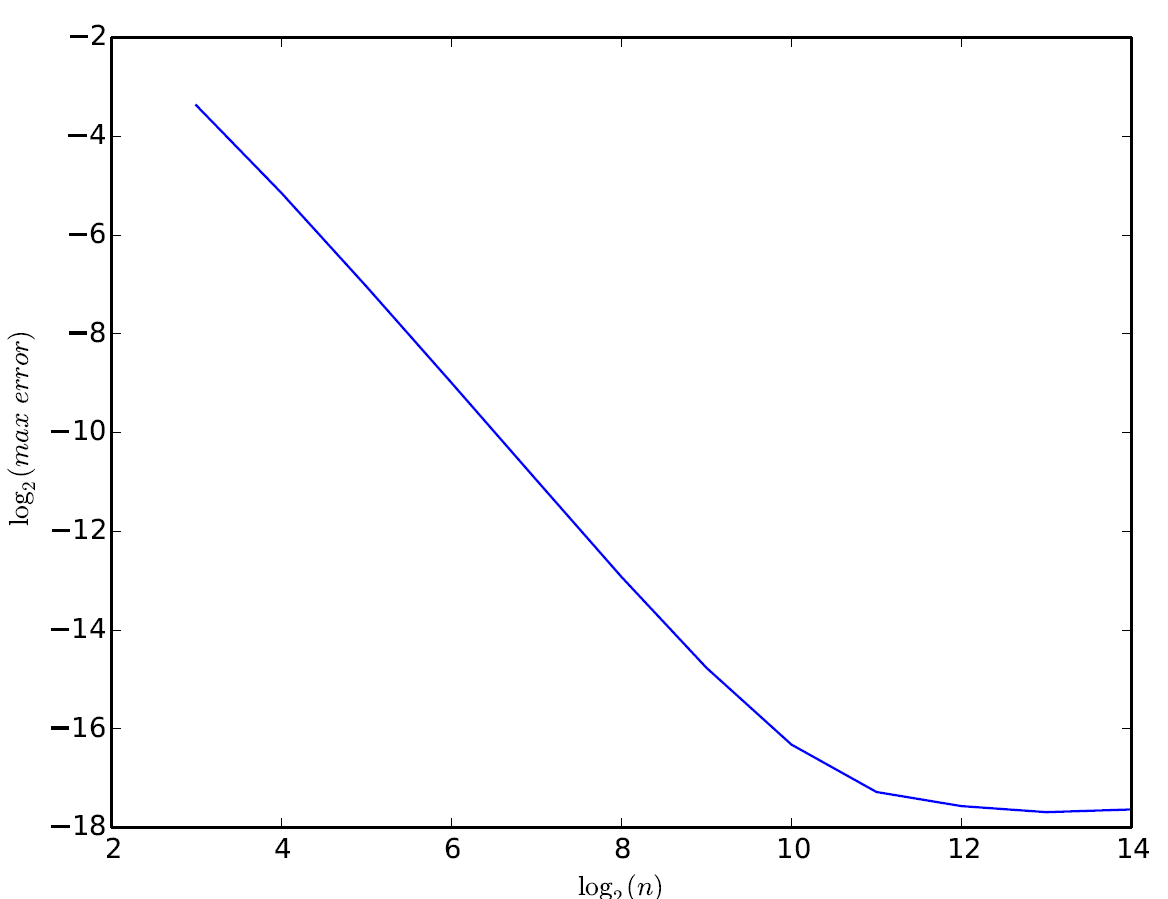
\includegraphics[width=0.7\linewidth]{bilder/error}
		\caption{The plot is produced by the python script on our \href{https://github.com/erikfsk/Project-1}{github}. It runs the main.cpp program and checks the max error for different n-values.}
		\label{fig:error}
	\end{figure}

















\section{Discussion}
















\section{Conclusion}
The specific solution is the fastest, but if the matrix have a slight change it does not solve the problem we have. The general is almost as fast, but it can solve a wider range of tridiagonal matrices. The LU solution is the slowest. It is useful no matter what matrix you have, but it has a significant drawback in speed. By our calculations the error is the same for every method. The error seem to follow until a point where the error become bigger for smaller steps. 



















%\printbibliography

\end{document}